%%% lorem.tex --- 
%% 
%% Filename: lorem.tex
%% Description: 
%% Author: Ola Leifler
%% Maintainer: 
%% Created: Wed Nov 10 09:59:23 2010 (CET)
%% Version: $Id$
%% Version: 
%% Last-Updated: Wed Nov 10 09:59:47 2010 (CET)
%%           By: Ola Leifler
%%     Update #: 2
%% URL: 
%% Keywords: 
%% Compatibility: 
%% 
%%%%%%%%%%%%%%%%%%%%%%%%%%%%%%%%%%%%%%%%%%%%%%%%%%%%%%%%%%%%%%%%%%%%%%
%% 
%%% Commentary: 
%% 
%% 
%% 
%%%%%%%%%%%%%%%%%%%%%%%%%%%%%%%%%%%%%%%%%%%%%%%%%%%%%%%%%%%%%%%%%%%%%%
%% 
%%% Change log:
%% 
%% 
%% RCS $Log$
%%%%%%%%%%%%%%%%%%%%%%%%%%%%%%%%%%%%%%%%%%%%%%%%%%%%%%%%%%%%%%%%%%%%%%
%% 
%%% Code:

\chapter{Method}
\label{cha:method}

Forecasting electricity prices involves using historical electricity prices and relevant factors. Most commonly, the steps for EPF include the following:
\begin{enumerate}
    \item Data extraction: This step involves identifying and gathering important factors that influence electricity prices. The data should include historical data on electricity prices, calendar data such as holidays and weather conditions like temperature.
    \item Data processing: This step involves cleaning and normalizing the gathered data and converting it to a suitable format. In the case of calendar data which is considered as a categorical value, one-hot encoding can be used. 
    \item Model implementation: There are many ways to design a LSTM-model. This step involves designing and testing various implementations that work with the dataset. 
    \item Model training: This step is divided in training and testing phase which includes dividing the dataset where a training set is used to train the forecasting model.
    \item Model evaluation: This step evaluates the performance of the trained model using the test set and validation set. Suitable evaluation metrics included in this project are Mean Absolute Error (MAE), Root Mean Squared Error (RMSE), Mean Absolute Percentage Error (MAPE), and Symmetric Mean Absolute Percentage Error (SMAPE). 
    \item Forecasting: The final step is to use the best trained model to generate predictions and calculate the prediction interval.
\end{enumerate}

The following chapter goes into detail of the steps provided above. 

\section{Dataset}
The data used in this thesis includes market data from Nord Pool, weather data from the Swedish Meteorological and Hydrological Institute (SMHI) and production data from Svenska Kraftnät (SVK) supplied by SYSPower \cite{SKM}. The full dataset contains hourly observations covering the period from January 2019 to February 2024. The coverage period is approximately 5 years, similar to the study by Lago et al. \cite{LAGO2021116983}. 

\subsection{Nord Pool market data}
The target variable for prediction is the hourly day-ahead prices, measured in price per each megawatt-hours (SEK/MWh) for the SE3 zone. The price for the next day is published every day at approximately 14:00 CET. Table \ref{tab:spot} provides some descriptive statistics of the spot price from 2018 to 2023. 

\begin{table}[H]
    \centering
    \begin{tabular}{|l|llcll|}
    \hline
    Year  & Observations &  Mean &   Standard Deviation &     Minimum &      Maximum \\
    \hline
    2018 &  8759 &   457.77 &   126.85 &   16.65 &  2573.41 \\ 
    2019 &  8759 &   405.49 &   107.00 &    1.28 &  1122.79 \\
    2020 &  8783 &   221.04 &   198.94 &  -17.92 &  2584.07 \\
    2021 &  8759 &   671.66 &   610.00 &  -20.00 &  6458.81 \\
    2022 &  8759 &  1378.79 &  1373.56 &  -22.35 &  8513.26 \\
    2023 &  8759 &   589.79 &   514.54 & -690.49 &  3758.65 \\
    \hline
    \end{tabular}
    \caption{Descriptive statistics for yearly spot prices, SE3 bidding zone. }
    \label{tab:spot}
\end{table}

The day-ahead transmission capacity is the amount of electricity that can be transmitted from one bidding zone to another. It is published at 10:00 CET the day before delivery and is measured in megawatt-hours (MWh)\cite{NordPool_capacities}. Transmission capacities into SE3 from neighbouring zones was extracted as it shows how the price in SE3 is affected by relying on neighbouring zones.

Electricity consumption in megawatt-hours (MWh) was included for all zones in Sweden. The consumption of electricity is an indicator for demand which affects the price. 

\subsection{Weather data}
As discussed in chapter \ref{cha:theory}, weather conditions impact both supply and demand. Temperature is known to affect the demand for electricity where for instance more electricity is used for heating during colder periods. As hydropower and wind power were together responsible for over 60\% of the total generation in 2023, precipitation and wind velocity affect the production of electricity as well. 

For this reason, the dataset includes temperature measured in Celsius (C), precipitation energy in megawatt-hours (MWh) and wind speed in meters per second (m/s). Due to availability, the measurements for temperature were collected as daily averages over Sweden. For wind speed, hourly measurements from five weather stations were selected due to their vicinity to wind parks and population centers \cite{windstats}. These five weather stations are Piteå, Malmö, Västmarkum, Junsele and Stockholm. Lastly, for precipitation energy the data is provided directly by SYSPower as daily average over Sweden. 

\subsection{Production data}
The production data is provided by SVK and is separated by production source. Figure \ref{fig:prodbytype} shows a box plot of the amount of electricity produced by each production source during the period 2018-2023.

\begin{figure}[H]
    \centering
    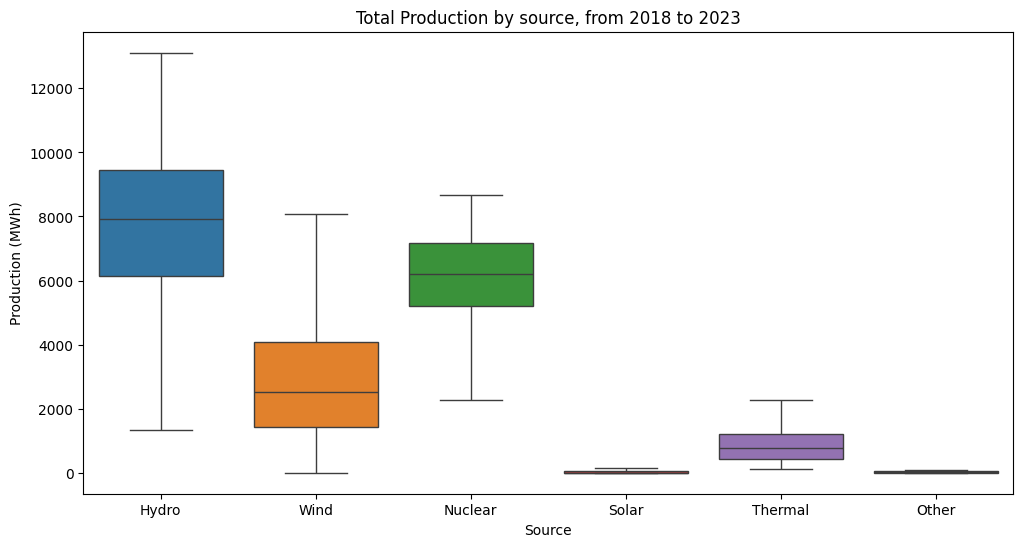
\includegraphics[height=8cm, width=0.85\textwidth]{figures/production_by_type.png}
    \caption{Production (MWh) in y-axis separated by production source in x-axis.} 
    \label{fig:prodbytype}
\end{figure}

\subsection{Calendar information}
To capture the effects of seasonality, the following categorical variables to represent calendar information were created:

\begin{itemize}
    \item \textit{Hour}: This variable takes values in range $0, 1, \dots, 23$ which represents the hour of the day.
    \item \textit{Day of week}: This variable takes values in the range $1, 2, \dots, 7$ representing weekdays and weekends. 
    \item \textit{Month}: This variable takes values in the range $1, 2, \dots, 12$ representing month of the year. 
    \item \textit{Year}: This variable takes values in the range $2018, 2019, \dots, 2024$ representing the year. 
    \item \textit{Holiday}: This variable is binary to represent holidays.
\end{itemize}

The above variables were encoded using one-hot-encoding which is a common way of encoding categorical information into suitable format \cite{WAGNER2022100246}. 

\subsection{Pre-processing}
Data preprocessing is carried out with the goal of having a complete dataset in suitable format to use for model training. The chosen variables for this study do suffer from missing values ranging from less than 1\% to approximately 5\% of the total number of rows. To avoid the loss of information and keep the temporal structure of the dataset, the rows with missing values were imputed using linear interpolation. 

For neural networks, feature scaling is usually applied to the input data to help speed up training time and improve performance \cite{coupling}. The dataset was normalized using min-max normalization. The min-max normalization is a linear transformation defined by: 

\begin{equation}
    X' = \frac{X - X_{min}}{X_{max} - X_{min}}
\end{equation}

where $x_{min}$ and $x_{max}$ are the minimum and maximum values of the feature $X$. 

\section{Feature selection}
To analyze the most important features that affect the electricity price, the Pearson correlation coefficient was used to measure the linear relationship between the price and feature. Given two variables (X,Y) the Pearson correlation coefficient is given by:

\begin{equation}
    \frac{cov(X,Y)}{\sigma_{X}\sigma_{Y}}
\end{equation}

Where the the covariance of the two variables X and Y are divided by the product of their
standard deviations. The result is a value between -1 and 1. Correlation equal to 1
implies perfect correlation and -1 perfect negative correlation, while a value of 0 implies no correlation between the dependent variables. 

\section{Dimensionality reduction}
As there are many features that are considered, the risk of overfitting and the curse of dimensionality increases \cite{goodfellow}. Therefore, principal component analysis (PCA) \cite{goodfellow} will be used to reduce the number of dimensions to mitigate the consequences of a large dataset with many features. The steps to perform PCA are as follows \cite{goodfellow}:

\begin{enumerate}
    \item Feature standardization: It is essential to standardize the feature to have zero-mean and unit-variance. This can be done with equation \ref{eq:zscore}. 
    \begin{equation}\label{eq:zscore}
        x' = \frac{x-\bar{x}}{\sigma}
    \end{equation}
    Where x is the feature vector, $\bar{x}$ is the mean of the feature vector and $\sigma$ is its standard deviation. 
    \item Covariance: Calculate the covariance matrix of the standardized input $x'$.
    \item Eigenvalue and eigenvector: Calculate the eigenvalues and eigenvectors of the covariance matrix. 
    \item Selecting principal components: Select the top $k$ eigenvectors corresponding to the largest eigenvalues. These represent the most important principal components.
\end{enumerate}

Note that PCA is not a feature selection method, as it produces components from combinations of the original data. PCA was applied to the pre-processed dataset, where the number of principal components were selected so that the sum of the explained variance was at 90\%. This indicates that 90\% of the information in the original dataset is covered by the principal components.  

\subsection{Training, validation and test split}
The dataset was divided into three parts; the training, validation and test sets \cite{goodfellow}. The training set is used to train the model and the validation set is used to evaluate the model's performance according to an arbitrary loss function. Finally, the test set is completely independent and is used to asses the final performance of the trained model. The purpose of the test set is to measure how well the model performs on unseen data. Furthermore, there is no overlap between the three sets which helps against overfitting \cite{nielsen}. 
\\\\
The training set ranges from January 1st 2018 to December 2021. The validation ranges from January 2022 to December 2022. Finally, the test set ranges from January 2023 to February 2024. The length of the validation and test set was chosen so that all seasons of the year are considered. Note that the selected ranges will not be used for cross-validation (CV), where the data is instead split into disjoint partitions where each possible partition is used once as the test set with the remaining data as the training set to find the model that performs the best across all partitions \cite{LAGO2021116983}. 

\section{LSTM models}
Once the dataset has been pre-processed, transformed into a suitable format and split into the training, validation and test sets it can be used to train the model. 
\\\\
The LSTM models implemented in this thesis are inspired by related studies from Jana \& Paul \cite{stackedlstm}, Ugurlu et al. \cite{architechture1}, Lehna et al. \cite{arch2} and Abdellatif et al. \cite{bilstm}. The first network architecture is a single-layer network, i.e one LSTM layer and a final fully connected layer for prediction. The second architecture consists of four layers: two LSTM layers, a flatten layer to flatten the output, followed by two dense layers where the final dense layer is used for prediction \cite{stackedlstm, arch2}. The third architecture is a bidirectional LSTM (BiLSTM) \cite{bilstm} which essentially adds another LSTM layer with reversed direction of the information flow \cite{diveLSTM}. This allows the layer to preserve information from both past and future, compared to the standard LSTM which only considers past information \cite{diveLSTM}. 

\subsection{Loss function}
A loss function is essentially a method of evaluating how well the model performs on the dataset, which in turn is minimized by the optimizer. The most common loss functions based on related studies \cite{architechture1, QRA, arch2, stackedlstm} are MAE as defined by equation \ref{eq:mae} and Mean Squared Error (MSE) which is given by:

\begin{equation}
    {\frac{1}{m} \sum_{j=1}^m  {(\hat{y}_{i}-y_{i})}^2}
\end{equation}

where $m$ is the number of samples, $\hat{y}_{i}$ is the predicted value and $y_{i}$ is the actual value. Both loss functions were used to evaluate the accuracy of the three models. 

\subsection{Multi-step forecasting}
After training the model, prediction is performed one-step ahead where one step is one hour. More specifically, the network state is initialized by predicting on the validation set first. To forecast 5 days or 120 hours ahead, one time step forecasting at a time is performed. Prediction of the first test sample is made once training is finished, which in turn is utilized to update the network state \cite{zhang}. Subsequent predictions are performed on the test sample for the remaining 119 steps. 

\subsection{Hyperparameter selection and optimization}
Hyperparameters are model parameters that are set before model training. Hyperparameter selection and tuning is a complex process in DL because of high numbers of possible combinations, and experimenting with large the number of combinations is computationally expensive. Model parameters of importance to this thesis include:

\begin{itemize}
    \item The number of neurons in the LSTM layer and the dense layer. 
    \item The number of samples that will be propagated through the network, i.e batch size. A larger batch size requires less training time, while a smaller batch size lets the model generalize better \cite{batchSize}. 
    \item Activation function applied to the LSTM layer and the dense layer. The ReLU activation function is a good default choice for the dense layer according to Goodfellow et al. \cite{goodfellow}, while for the LSTM layer the standard choice is $tanh$ \cite{diveLSTM}.
    \item Regularization techniques such as the dropout layer, L1 and L2 regularization. Dropout prevents overfitting by deactivating a proportion of neurons in a layer at random, helping the model to generalize better on the dataset \cite{goodfellow}. L1 and L2 regularization add a penalty term which helps filter out less important features in the model to zero \cite{diveLSTM}. 
    \item The optimizer used for model training. The optimizers tested were Adam \cite{adam, goodfellow} and Root Mean Square Propagation (RMSProp) \cite{goodfellow}. 
    \item The step size at which the optimizer updates the weights during model training, i.e the learning rate. An appropriate learning rate makes training more efficient \cite{goodfellow}. 
    \item The loss function, i.e. a measurement of model performance to minimize. The two common loss functions for EPF is MSE and MAE \cite{diveLSTM}. 
    \item The number of training epochs. Epochs define the number of times the model will iterate through the entire training dataset \cite{nielsen}. Increasing the number of epochs gives the model more training opportunities, but increases computational cost and risks overfitting \cite{goodfellow}. 
    \item The sequence length. For LSTM, each input value is modeled as a sequence of past input values. Values too far in the past do not have any affect on the short-term future, with the worst case being a negative affect on training performance. This means that selecting the right length of the input sequence can help improve performance. 
\end{itemize}

To find the best combination of hyperparameters is important in order to improve performance, but it can also become exhaustive. For this reason, a method known as grid search \cite{gridSearch} was used which defines a search space for hyperparameters to find the best combination \cite{gridSearch, diveLSTM}. Grid search was applied on the following hyperparameters: the number of neurons, the batch size, activation function, learning rate, number of training epochs, the loss function, and the optimizer. To reduce and prevent overfitting, all three regularization techniques were implemented when necessary. To perform the grid search, a search space was set up as shown in Table \ref{tab:hyperparams}.

\begin{table}[H]
  \caption{Hyper-parameter search space}
  \label{tab:hyperparams}
  \centering
  \begin{tabular}{ll}
    \hline
    Parameter & Values \\
    \hline
    Input sequence & [120, 240] \\
    Batch Size & [8, 16, 32] \\
    Activation function & [tanh, ReLU] \\
    LSTM layer neurons & [8, 16, 32, 64, 128, 256, 512] \\
    Dense layer neurons & [8, 16, 32, 64, 128, 256, 512] \\
    Dropout rate & [0, 0.1, 0.2, 0.3, 0.4, 0.5] \\
    Learning rate & [0.01, 0.001, 0.0001] \\
    Loss function & [MSE, MAE] \\
    Optimizer & [Adam, RMSprop] \\
    \hline
  \end{tabular}
\end{table}

\subsection{Evaluation metrics}
Different evaluation metrics are employed to evaluate the accuracy of point forecasts. Common metrics for EPF include MAE (\ref{eq:mae}), RMSE (\ref{eq:rmse}), MAPE (\ref{eq:mape}) and SMAPE (\ref{eq:smape}) \cite{LAGO2021116983}. Given the number of samples $m$, the actual value $y_{i}$ and the predicted value $\hat{y_{i}}$ the four metrics can be formulated as follows: 

\begin{equation}\label{eq:mae}
    \frac{1}{m} \sum_{j=1}^m |(\hat{y}_{i}-y_{i})|
\end{equation}

\begin{equation}\label{eq:rmse}
    \sqrt{\frac{1}{m} \sum_{j=1}^m  {(\hat{y}_{i}-y_{i})}^2}
\end{equation}

\begin{equation}\label{eq:mape}
    \frac{100}{m} \sum_{j=1}^m |\frac{\hat{y}_{i}-y_{i}}{y_{i}}|
\end{equation}

\begin{equation}\label{eq:smape}
    \frac{100}{m}\sum_{j=1}^m \frac{|\hat{y}_{i} - y_{i}|}{(|y_{i}| + |\hat{y}_{i}|)/2}
\end{equation}

Each metric above has their advantages and drawbacks. MAE is generally robust to outliers compared to RMSE as it does not involve squaring but RMSE fails to penalize large errors. MAPE and SMAPE on the other hand provide a more relative measure to the true value compared to MAE. MAPE is asymmetric, which means that the error is higher if the forecast is higher than the actual value and error is lower when the forecast value is less than the actual value. SMAPE is a symmetric variation of MAPE that takes into account the scale of the values by using the average of the absolute values of the forecast and actual values in the denominator, which treats over- and under estimations with equal weight. 




%%%%%%%%%%%%%%%%%%%%%%%%%%%%%%%%%%%%%%%%%%%%%%%%%%%%%%%%%%%%%%%%%%%%%%
%%% lorem.tex ends here

%%% Local Variables: 
%%% mode: latex
%%% TeX-master: "demothesis"
%%% End: 
